\section{Drag and Drop}
\label{sec:implementationdraganddrop}
As mentioned in \secref{sec:androiddraganddrop}, the implementation of drag and drop has been simplified after SDK 11. This allows for an easy implementation of the drag and drop functionality. Before the explanation of drag and drop, we will first show the hierarchy of the layouts on the station and the wagons.
\begin{figure}[H]
\centering
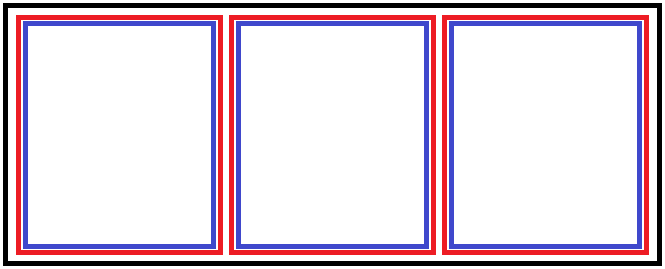
\includegraphics[width=0.9\linewidth]{img/layoutexample.png}%0.1 margin
\caption{Example of a LinearLayout container.}
\label{fig:linearlayoutcontainer}
\end{figure}
There are two LinearLayout containers on each station, and there are a LinearLayout containers on each wagon. An example of the LinearLayout container is shown in \autoref{fig:linearlayoutcontainer}. The black color represents the LinearLayout, the red color represents a Framelayout, and the blue color represents a pictogram. Each pictogram has attached an OnTouchListener, and each FrameLayout has attached an OnDragListener. Our TouchListener is shown below.

\begin{lstlisting}[language=java,firstnumber=1,caption={Our TouchListener},label=lst:ourtouchlistener] 
private final class TouchListener implements OnTouchListener {
	@Override
	public boolean onTouch(View view, MotionEvent motionEvent) {
		if (motionEvent.getAction() == MotionEvent.ACTION_DOWN) {
			ClipData data = ClipData.newPlainText("", "");
			DragShadowBuilder shadowBuilder = new View.DragShadowBuilder(view);
			view.startDrag(data, shadowBuilder, view, 0);
			view.setVisibility(View.INVISIBLE);
			return true;
		}
		else if (motionEvent.getAction() == MotionEvent.ACTION_UP) {// prevents that a pictogram disappears if only pressed and no drag
			if(view != null && view.getVisibility() == View.INVISIBLE){
				view.setVisibility(View.VISIBLE);
			}
			return true;
		}
		else {
			return false;
		}
	}
}
\end{lstlisting}
\begin{description}
\item[Line 3] The \lstinline|onTouch()| method is called when the pictograms receives a touch input.
\item[Lines 4-7] If the touch event is a press motion, make a view shadow, and start the drag.
\item[Line 8] Set the pictogram's visibility to invisible.
\item[Lines 11-14] If the touch event is a release motion and the pictogram is invisible, then make the pictogram visible. This if sentence was added since it was possible to make the pictogram disappear with only a press motion.
\todo{Der er nødt til at stå hvorfor den returnerer true/false}
\end{description}
When the method \textit{view.startDrag()} is called, the OnDragListener event is fired. Our OnDragListener is shown below.
\begin{lstlisting}[language=java,firstnumber=1,caption={Our DragListener},label=lst:ourdraglistener] 
private class DragListener implements OnDragListener {
	public boolean onDrag(View hoverView, DragEvent event) {
	    View draggedView = (View) event.getLocalState();
		switch (event.getAction()) {
			case DragEvent.ACTION_DROP:
				// DropAction, assigns the draggedview to the dropContainer if, the dropContainer does not already contain a pictogram.
				ViewGroup ownerContainer = (ViewGroup) draggedView.getParent();
				PictoFrameLayout dropContainer = (PictoFrameLayout) hoverView;
				Object tag = hoverView.getTag();
				if (tag == null) {
					ownerContainer.removeView(draggedView);
					ownerContainer.setTag(null);
					dropContainer.addView(draggedView);
					dropContainer.setTag("filled");
				}
				draggedView.setVisibility(View.VISIBLE);
				break;

			case DragEvent.ACTION_DRAG_ENDED:
				// Makes the draggedview visible again after the view has been moved or if drop wasn't valid.
				if(event.getResult() == false){
					draggedView.setVisibility(View.VISIBLE);
				}
				break;
		}
		return true;
	}
}
\end{lstlisting}
\begin{description}
\item[Line 2] The \lstinline|onDrag()| method is called when a pictogram starts being dragged.
\item[Line 3] Get the current dragged pictogram and initialize the variable \lstinline|draggedView|.
\item[Line 4] Switch case of the current drag event.
\item[Line 5] Case if the current drag event is dropping the pictogram on a FrameLayout.
\item[Lines 7-8] Initialize the variable \lstinline|ownerContainer| with the parent Framelayout of the dragged pictogram, and initialize variable \lstinline|dropContainer| with the FrameLayout currently being hovered above.  
\item[Lines 9-10] Initialize the variable \textit{tag} with the current status of the \lstinline|dropContainer|, if the status is "filled" then the \lstinline|dropContainer| is already containing a pictogram, and is therefore not eligible for the drop.
\item[Lines 11-16] If the \lstinline|dropContainer| does not contain a pictogram, then the pictogram can be moved from \lstinline|ownerContainer| to \lstinline|dropContainer|. The tag in \lstinline|ownerContainer| is set to \lstinline|null| and the tag in \lstinline|dropContainer| is set to \lstinline|"filled"|, to indicate to it now contains a pictogram. The \lstinline|draggedView| becomes visible after a drop.
\item[Line 19] If current drag event is drag ended,  there were not performed a valid drop the \lstinline|draggedView| will become visible again. This will make it look like the pictogram snaps back to its position, since the drop was not valid.
\end{description}
Some cases has been excluded in \autoref{lst:ourdraglistener} because they are not relevant for the functionality of the drag and drop.
